\documentclass[a4paper]{article}

\usepackage{pdflscape}
\usepackage{multicol}
\usepackage{blindtext}
\usepackage{color}
\usepackage{enumitem}

\usepackage[left=10mm, right=10mm, top=10mm, bottom=10mm]{geometry}

\usepackage{titlesec}

\usepackage[utf8]{inputenc}
\usepackage{fourier} 
\usepackage{array}
\usepackage{makecell}

\usepackage[demo]{graphicx}



\renewcommand\theadalign{bc}
\renewcommand\theadfont{\bfseries}
\renewcommand\theadgape{\Gape[4pt]}
\renewcommand\cellgape{\Gape[4pt]}

\titlespacing\section{0pt}{5pt plus 4pt minus 2pt}{0pt plus 2pt minus 2pt}
\titlespacing\subsection{0pt}{5pt plus 4pt minus 2pt}{0pt plus 2pt minus 2pt}
\titlespacing\subsubsection{0pt}{5pt plus 4pt minus 2pt}{0pt plus 2pt minus 2pt}

\newenvironment{Figure}
  {\par\medskip\noindent\minipage{\linewidth}}
  {\endminipage\par\medskip}


\setlength{\columnseprule}{0.5pt}
\def\columnseprulecolor{\color{black}}

\pagenumbering{gobble}

\title{MuDa Cheat Sheet}
\author{Niklas Ullmann}
\date{Summer 2022}

%

\begin{document}
\begin{landscape}
    \thispagestyle{empty}

    \begin{multicols}{4}
        \section{Grundlagen}
        \begin{itemize}[noitemsep,nolistsep,leftmargin=*]
            \item Grundlagen
            \begin{itemize}[noitemsep,nolistsep,leftmargin=*]
                \item\textbf{ $Y = f(x) + \epsilon$}
                \item $Y$ = Zielgröße, $f()$ = unbekanntes/wahres Modell, $X$ = Prädiktoren, $\epsilon$ Nicht reduzierbarer Fehler
                \item \textbf{$\hat{Y} = \hat{f}(X)+\epsilon$}
                \item $\hat{Y}$ = Schätzung der Zielgröße, $\hat{f}$ = Schätzung des Modells
                \item Ziel: Möglichst genaue Schätzung finden
            \end{itemize}
            \item Bias-Variance Tradeoff
            \begin{itemize}[noitemsep,nolistsep,leftmargin=*]
                \item Bias:
                \item Variance:
            \end{itemize}
            
            
        \end{itemize}
        \begin{Figure}
            \centering
            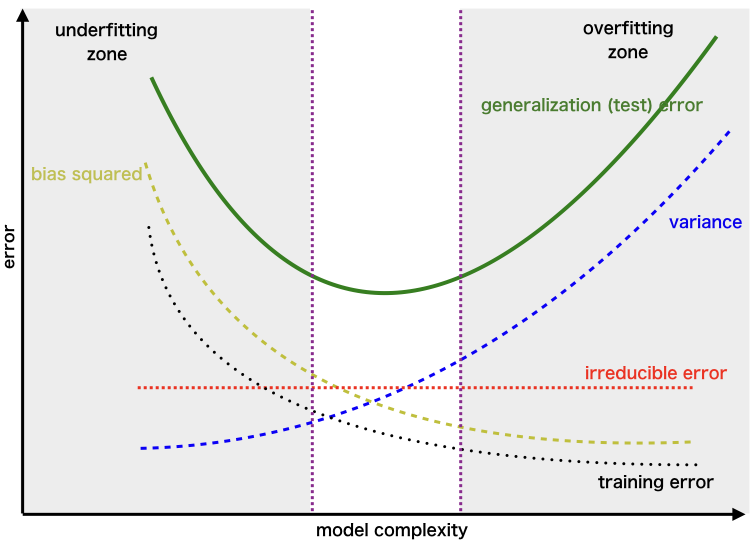
\includegraphics[width=\linewidth]{bv_tradeoff.png}
        \end{Figure}

        \section{Regression}
        \section{Klassifikation}
        \section{Resampling}
        \section{Modellauswahl}
        \section{R - Hilfe}
        \section{Other}

    
    \end{multicols}
    
\end{landscape}
\end{document}